\documentclass[sigconf]{acmart}

\usepackage{graphicx}
\usepackage{amsmath}
% 避免 \Bbbk 重复定义冲突
\let\Bbbk\relax
\usepackage{amssymb}
\usepackage{booktabs}
\usepackage{algorithm}
\usepackage{algpseudocode}
\usepackage{xcolor}
\usepackage{listings}

\lstset{
    basicstyle=\ttfamily\small,
    keywordstyle=\color{blue},
    commentstyle=\color{green!60!black},
    stringstyle=\color{red},
    showstringspaces=false,
    breaklines=true,
    frame=single,
    numbers=left,
    numberstyle=\tiny\color{gray},
    captionpos=b
}

\title{Final Report of Image Rendering}

\author{Hengxu Wu}
\affiliation{
  \institution{2024011308, Yao Class 43}
  \city{Beijing}
  \country{China}
}
\email{wuhx24@mails.tsinghua.edu.cn}

\begin{abstract}
This report presents the final results of our GPU-based image rendering system project. The system implements a complete rendering pipeline with support for advanced shading techniques, including Phong illumination model, texture mapping and multiple materials. We have successfully developed the core architecture, implemented key rendering algorithms, and achieved great performance for moderately complex scenes. Furthermore, we have integrated advanced visual effects such as Cartoonization, Relativistic Rendering, Chromatic Dispersion, and Depth of Field. This document details our technical approach, final achievements, challenges encountered, and future development possibilities.
\end{abstract}

\keywords{Computer Graphics, GPU Rendering, Shading, Texture Mapping, Real-time Rendering}

\begin{document}

\maketitle

\section{Introduction}
This project aims to architect a high-performance rendering system purely on GPU using DirectX12. Unlike traditional approaches that rely on pre-existing frameworks, we are building the entire pipeline from scratch to ensure maximum control and optimization.

Our system supports multiple model formats including OBJ, glTF, FBX, and Blend. It features a GPU-based path tracing renderer that implements acceleration structures, material evaluation, and light sampling. For image quality improvement, we have integrated Intel Open Image Denoise~\cite{OpenImageDenoise} and implemented various special effects including Cartoonization, Relativistic Rendering, Chromatic Dispersion, and Depth of Field. The repository for this project can be found at: \url{https://github.com/gameswu/acg_project}.

\section{Method}

\subsection{Overall Architecture}
We have implemented a high-performance rendering system purely on GPU using DirectX12. Unlike traditional approaches that rely on pre-existing frameworks, building the entire pipeline from scratch ensures maximum control and optimization.

The system architecture is structured to support scalability and high performance. As shown in Figure~\ref{fig:arch_new}, the pipeline consists of three main stages: Conversion, Rendering, and Processing. In the conversion stage, our Python-based pipeline standardizes various model formats (OBJ, FBX, glTF) into our efficient binary format (.acg) to support uniform material parsing.

\begin{figure}[h]
    \centering
    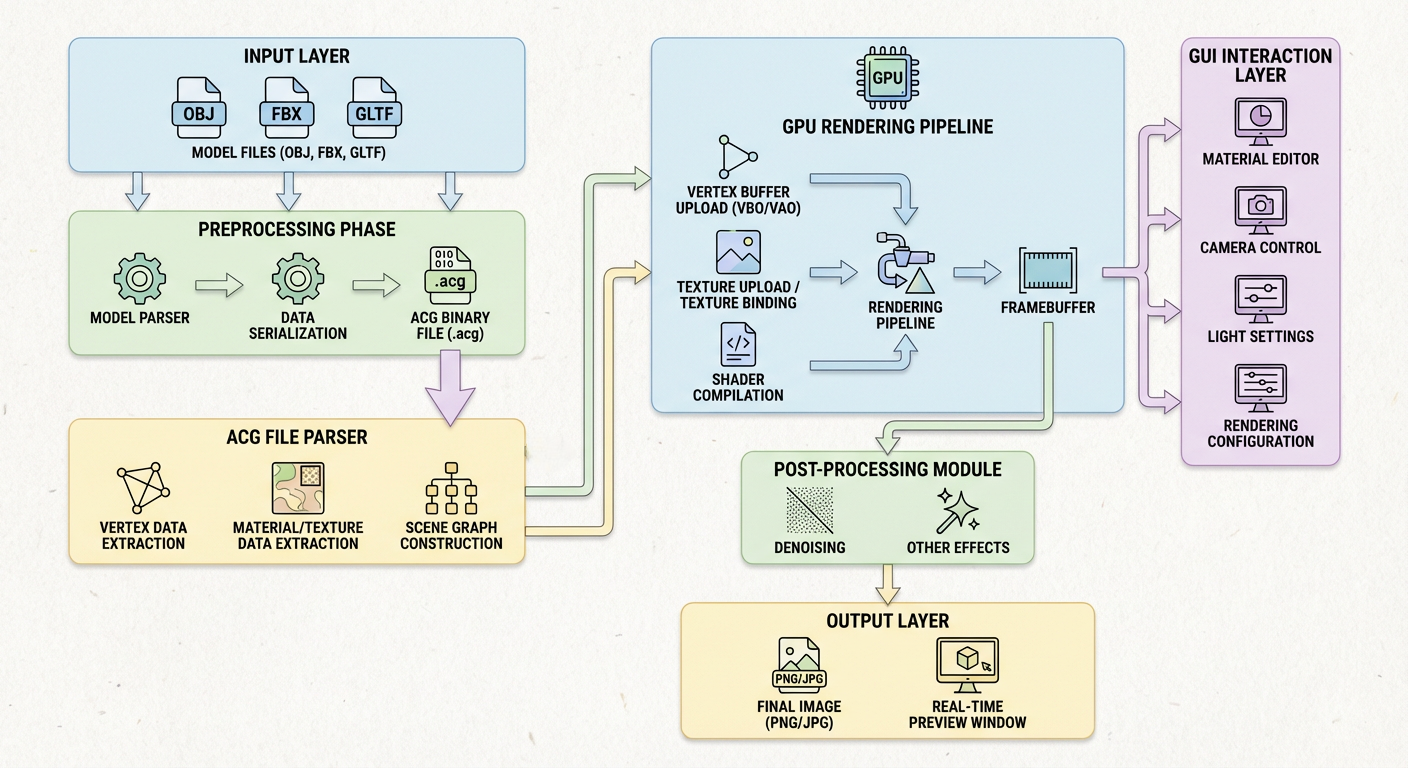
\includegraphics[width=0.9\linewidth]{../slide/fig/archi.png}
    \caption{System Architecture Diagram}
    \label{fig:arch_new}
\end{figure}

\subsubsection{Path Tracing Kernel}
The core of our renderer is a physical-based path tracer that solves the rendering equation:
\begin{equation}
L_o(p, \omega_o) = L_e(p, \omega_o) + \int_{\Omega} f_r(p, \omega_i, \omega_o) L_i(p, \omega_i) \cos\theta_i d\omega_i
\end{equation}
where $L_e$ represents emitted radiance, and $f_r$ is the BRDF.

We implement an iterative path tracing loop in HLSL (Algorithm~\ref{alg:pathtracing}). For each bounce, we find the nearest intersection, evaluate emission, and then sample the next direction based on the material's BSDF. The system also supports Image-Based Lighting (IBL) using skyboxes. The infinite environment light is sampled as part of the path tracing process: when a ray escapes the scene, the `SampleEnvironment` function queries the skybox texture to contribute to the background radiance and scene lighting. To prevent infinite recursion, we employ Russian Roulette termination when the path depth exceeds a threshold.

\begin{algorithm}[H]
\caption{Path Tracing with Russian Roulette}
\begin{algorithmic}[1]
\State $radiance \gets 0$
\State $throughput \gets 1$
\For{$bounce = 0$ to $maxBounces$}
    \State $hit \gets TraceRay(ray)$
    \If{ not $hit.isIntersected$}
        \State $radiance \gets radiance + throughput \times SampleEnvironment(ray.dir)$
        \State \textbf{break}
    \EndIf
    \State $radiance \gets radiance + throughput \times hit.material.emission$

    \State $nextDir, pdf \gets SampleBSDF(hit, -ray.dir)$
    \State $throughput \gets throughput \times BSDF \times \cos\theta / pdf$

    \If{$bounce > 3$}
        \State $rrProb \gets \min(\max(throughput), 0.95)$
        \If{$Random() > rrProb$} 
            \State \textbf{break}
        \EndIf
        \State $throughput \gets throughput / rrProb$
    \EndIf
    \State $ray \gets CreateRay(hit.pos, nextDir)$
\EndFor
\end{algorithmic}
\label{alg:pathtracing}
\end{algorithm}

To balance noise from direct lighting and specular highlights, we utilize Multiple Importance Sampling (MIS) with the power heuristic ($\beta=2$):
\begin{equation}
w(p_i) = \frac{p_i(x)^\beta}{\sum_j p_j(x)^\beta}
\end{equation}
This combines probability densities from both light source sampling and BSDF sampling effectively.

\subsection{Advanced Materials}
Our renderer features a robust material system based on the Disney Principled BSDF model, integrating both diffuse and specular terms.
The Normal Distribution (NDF) uses the Trowbridge-Reitz GGX distribution to model microfacet roughness:
\begin{equation}
D(H) = \frac{\alpha^2}{\pi ((N \cdot H)^2 (\alpha^2 - 1) + 1)^2}
\end{equation}
where $\alpha = roughness^2$.
The Geometry Term employs the Smith model with Schlick-GGX approximation for shadowing and masking:
\begin{equation}
G(V, L) = G_1(V) G_1(L), \quad G_1(v) = \frac{N \cdot v}{(N \cdot v)(1 - k) + k}
\end{equation}
Finally, the Fresnel Term is approximated using Schlick's approximation:
\begin{equation}
F(\theta) = F_0 + (1 - F_0)(1 - \cos\theta)^5
\end{equation}

For layered materials (e.g., Clearcoat, Sheen, Subsurface Scattering), we implement a stack-based evaluation strategy (Algorithm~\ref{alg:material}). A stochastic approach is used to select or blend between layers (e.g., base and coating) to maintain physical correctness without excessive computational cost.

\begin{algorithm}[H]
\caption{Layered Material Evaluation}
\begin{algorithmic}[1]
\State $f \gets 0$
\If{$material.hasClearcoat$}
    \State $prob_{coat} \gets CalculateCoatSelectionProb(V, L)$
    \If{$Random() < prob_{coat}$}
        \State \Return $EvaluateClearcoat(hit, V, L) / prob_{coat}$
    \EndIf
\EndIf

\State $f_{base} \gets EvaluatePrincipledBSDF(hit, V, L)$

\If{$material.hasSheen$}
    \State $f_{base} \gets f_{base} + EvaluateSheen(hit, V, L)$
\EndIf

\If{$material.hasSSS$}
    \State $f_{base} \gets Lerp(f_{base}, EvaluateSSS(hit, V, L), material.subsurface)$
\EndIf

\State \Return $f_{base}$
\end{algorithmic}
\label{alg:material}
\end{algorithm}

\subsection{Large Scene Management}
To handle large scenes with high-resolution textures that exceed GPU memory, we implemented a Virtual Texture system based on sparse binding and tile-based indirect mapping.
This system operates on three principles. First, tiling splits large textures into $256 \times 256$ independent tiles. Second, an indirection table maps virtual UV coordinates to physical memory locations. Specifically, the physical UV is calculated as:
\begin{equation}
UV_{phys} = \frac{TilePos(ID) \cdot 256 + (UV_{virt} \cdot Size) \pmod{256}}{PoolSize}
\end{equation}
Third, demand loading ensures that the renderer detects missing tiles during execution and requests them from the disk.

\subsection{Chromatic Dispersion}
We simulate chromatic dispersion by accounting for the wavelength dependence of the refractive index.
First, a stochastic wavelength selection is performed where each refraction event randomly selects one of the R, G, or B channels.
Second, an index offset is applied based on the selected channel:
\begin{equation}
n_{red} = n_{base} \cdot (1 - S_{disp}), \quad n_{blue} = n_{base} \cdot (1 + S_{disp})
\end{equation}
where $S_{disp}$ is the dispersion strength.
Third, to ensure unbiased results, the path throughput is re-weighted by multiplying by 3 for the selected channel to compensate for the selection probability.

\subsection{Relativistic Rendering}
To simulate effects at relativistic speeds ($\beta = v/c \to 1$), we apply Lorentz transformations to light rays.
Aberration distorts the field of view as the camera moves. The ray direction angle $\theta$ is transformed to $\theta'$:
\begin{equation}
\cos(\theta') = \frac{\cos(\theta) - \beta}{1 - \beta \cos(\theta)}
\end{equation}
Doppler Shift changes the light frequency. The Doppler factor $D$ is defined as:
\begin{equation}
D = \gamma(1 + \beta \cos(\theta)), \quad f' = D \cdot f
\end{equation}
This is visualized by shifting RGB wavelengths and applying intensity falloff.
The Headlight Effect causes radiance to increase in the direction of motion:
\begin{equation}
I' = I \times D^2
\end{equation}

Algorithm~\ref{alg:relativity} summarizes how these relativistic factors modify both the ray geometry and its radiometric properties during the primary ray generation stage.

\begin{algorithm}[H]
\caption{Relativistic Ray Generation}
\begin{algorithmic}[1]
\State \textbf{Input:} Camera Ray direction $d$, Speed $\beta$
\State $\gamma \gets 1 / \sqrt{1 - \beta^2}$
\State $\cos\theta \gets \mathbf{dot}(d, \text{velocity\_dir})$
\State \Comment{Aberration: Update ray direction}
\State $\cos\theta' \gets (\cos\theta - \beta) / (1 - \beta \cos\theta)$
\State $d' \gets \text{ReconstructDirection}(d, \cos\theta')$ 

\State \Comment{Doppler \& Headlight Effect}
\State $D \gets \gamma (1 + \beta \cos\theta)$
\State $throughput \gets throughput \times D^2$ 
\State $ray.color \gets \text{ShiftWavelength}(ray.color, D)$

\State \Return $Ray(origin, d')$
\end{algorithmic}
\label{alg:relativity}
\end{algorithm}

\subsection{Depth of Field}
We utilize a Thin Lens model to simulate depth of field. The process involves multiple steps.
First, a focal point calculation determines the focal point $P_{focal}$ along the ideal pinhole ray given a focal distance $d_{focus}$.
Next, lens sampling selects a point $P_{lens}$ on the lens aperture disk of radius $R_{aperture}$.
Finally, ray re-direction constructs the new primary ray originating from $P_{lens}$ and targeting $P_{focal}$.
\begin{equation}
\omega_{new} = \text{Normalize}(P_{focal} - P_{lens})
\end{equation}

\subsection{Motion Blur}
Motion Blur is implemented by incorporating time as a dimension in the rendering equation.
This is implemented via time sampling, where each primary ray is assigned a random time $t \sim U[t_{start}, t_{end}]$ within the shutter interval.
Then, interpolation updates dynamic objects and the camera transform to the sampled time $t$ before intersection testing.
Finally, an accumulation step averages the radiance over many samples with different times, naturally producing the motion blur effect.

\subsection{Cartoonization}
The cartoon style is achieved through a post-processing pass.
The effect relies on posterization, where color values are quantized into discrete levels ($C_{step}$) to create flat shading areas.
\begin{equation}
C_{out} = \lfloor \frac{C_{in}}{C_{step}} \rfloor \cdot C_{step}
\end{equation}
Edge detection applies a Sobel filter to the image luminance using convolution kernels $K_x$ and $K_y$:
\begin{equation}
K_x = \begin{bmatrix} -1 & 0 & 1 \\ -2 & 0 & 2 \\ -1 & 0 & 1 \end{bmatrix}, \quad K_y = \begin{bmatrix} 1 & 2 & 1 \\ 0 & 0 & 0 \\ -1 & -2 & -1 \end{bmatrix}
\end{equation}
Pixels with a gradient magnitude $G = \sqrt{G_x^2 + G_y^2}$ exceeding a threshold are darkened to creating outlines.
Additionally, highlight preservation masks the edge detection in very bright areas to avoid dirtying specular highlights.

\subsection{Denoising \& Anti-Aliasing}
For denoising, we integrate the Intel Open Image Denoise (OIDN) library. It uses a deep learning-based approach to filter Monte Carlo noise from the rendered output. We provide albedo and normal buffers alongside the noisy color buffer to OIDN to preserve texture details and geometric edges during the denoising process.

For Anti-Aliasing, we use Sub-pixel Jittering (Temporal Anti-Aliasing). Instead of firing rays through the center of every pixel, we apply a sub-pixel offset $(\Delta x, \Delta y)$ to the raster coordinates for each frame. The final image is an average of these jittered frames:
\begin{equation}
I(x, y) = \frac{1}{N} \sum_{i=1}^{N} L(x + \Delta x_i, y + \Delta y_i)
\end{equation}
where $\Delta x_i, \Delta y_i \sim U[-0.5, 0.5]$ are random offsets. This converts aliasing artifacts (jaggies) into high-frequency noise, which converges to the correct anti-aliased integration over time.

\section{Results}

\subsection{Advanced Materials}
Our renderer successfully supports complex materials, including glass, metal, and layered materials. Figure~\ref{fig:cubes} shows different complex material cubes rendered in the scene, demonstrating the system's capability to handle sophisticated material properties. Additionally, Figure~\ref{fig:cubes2} illustrates the accurate rendering of Blender's Principled BSDF material.

\begin{figure}[h]
    \centering
    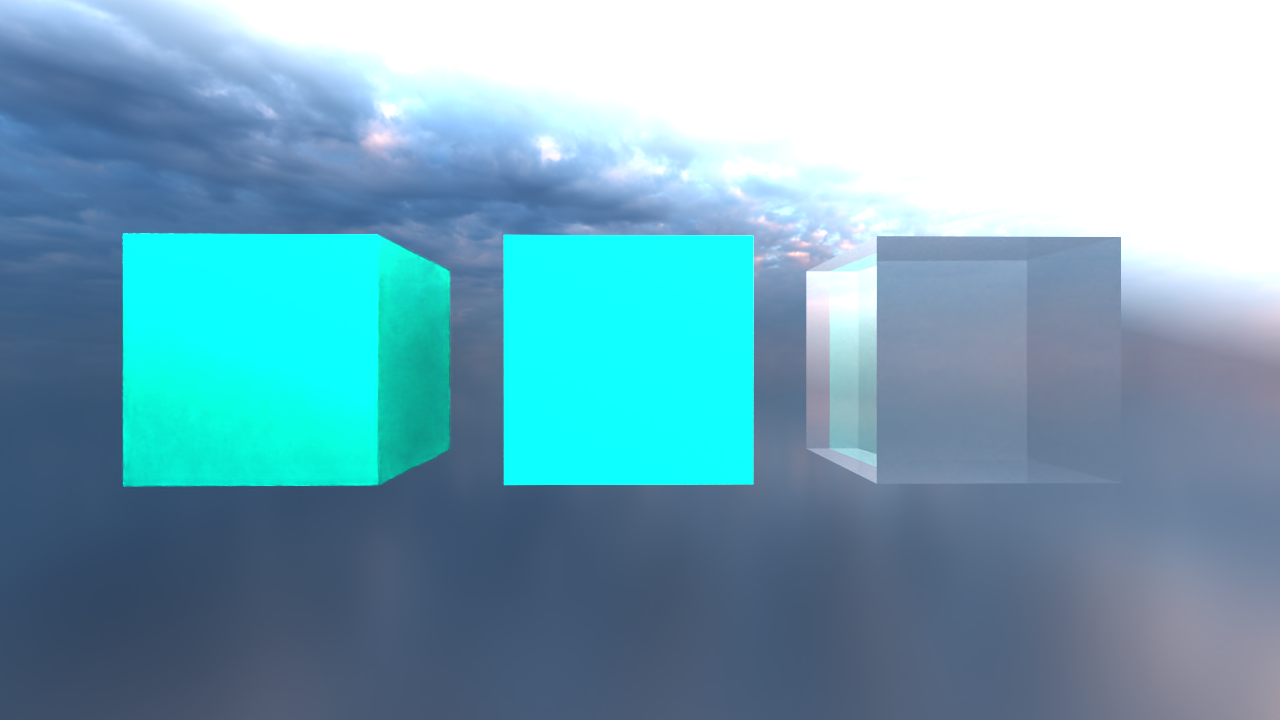
\includegraphics[width=0.8\linewidth]{../slide/fig/cubes.png}
    \caption{Advanced Materials: Complex material cubes}
    \label{fig:cubes}
\end{figure}

\begin{figure}[h]
    \centering
    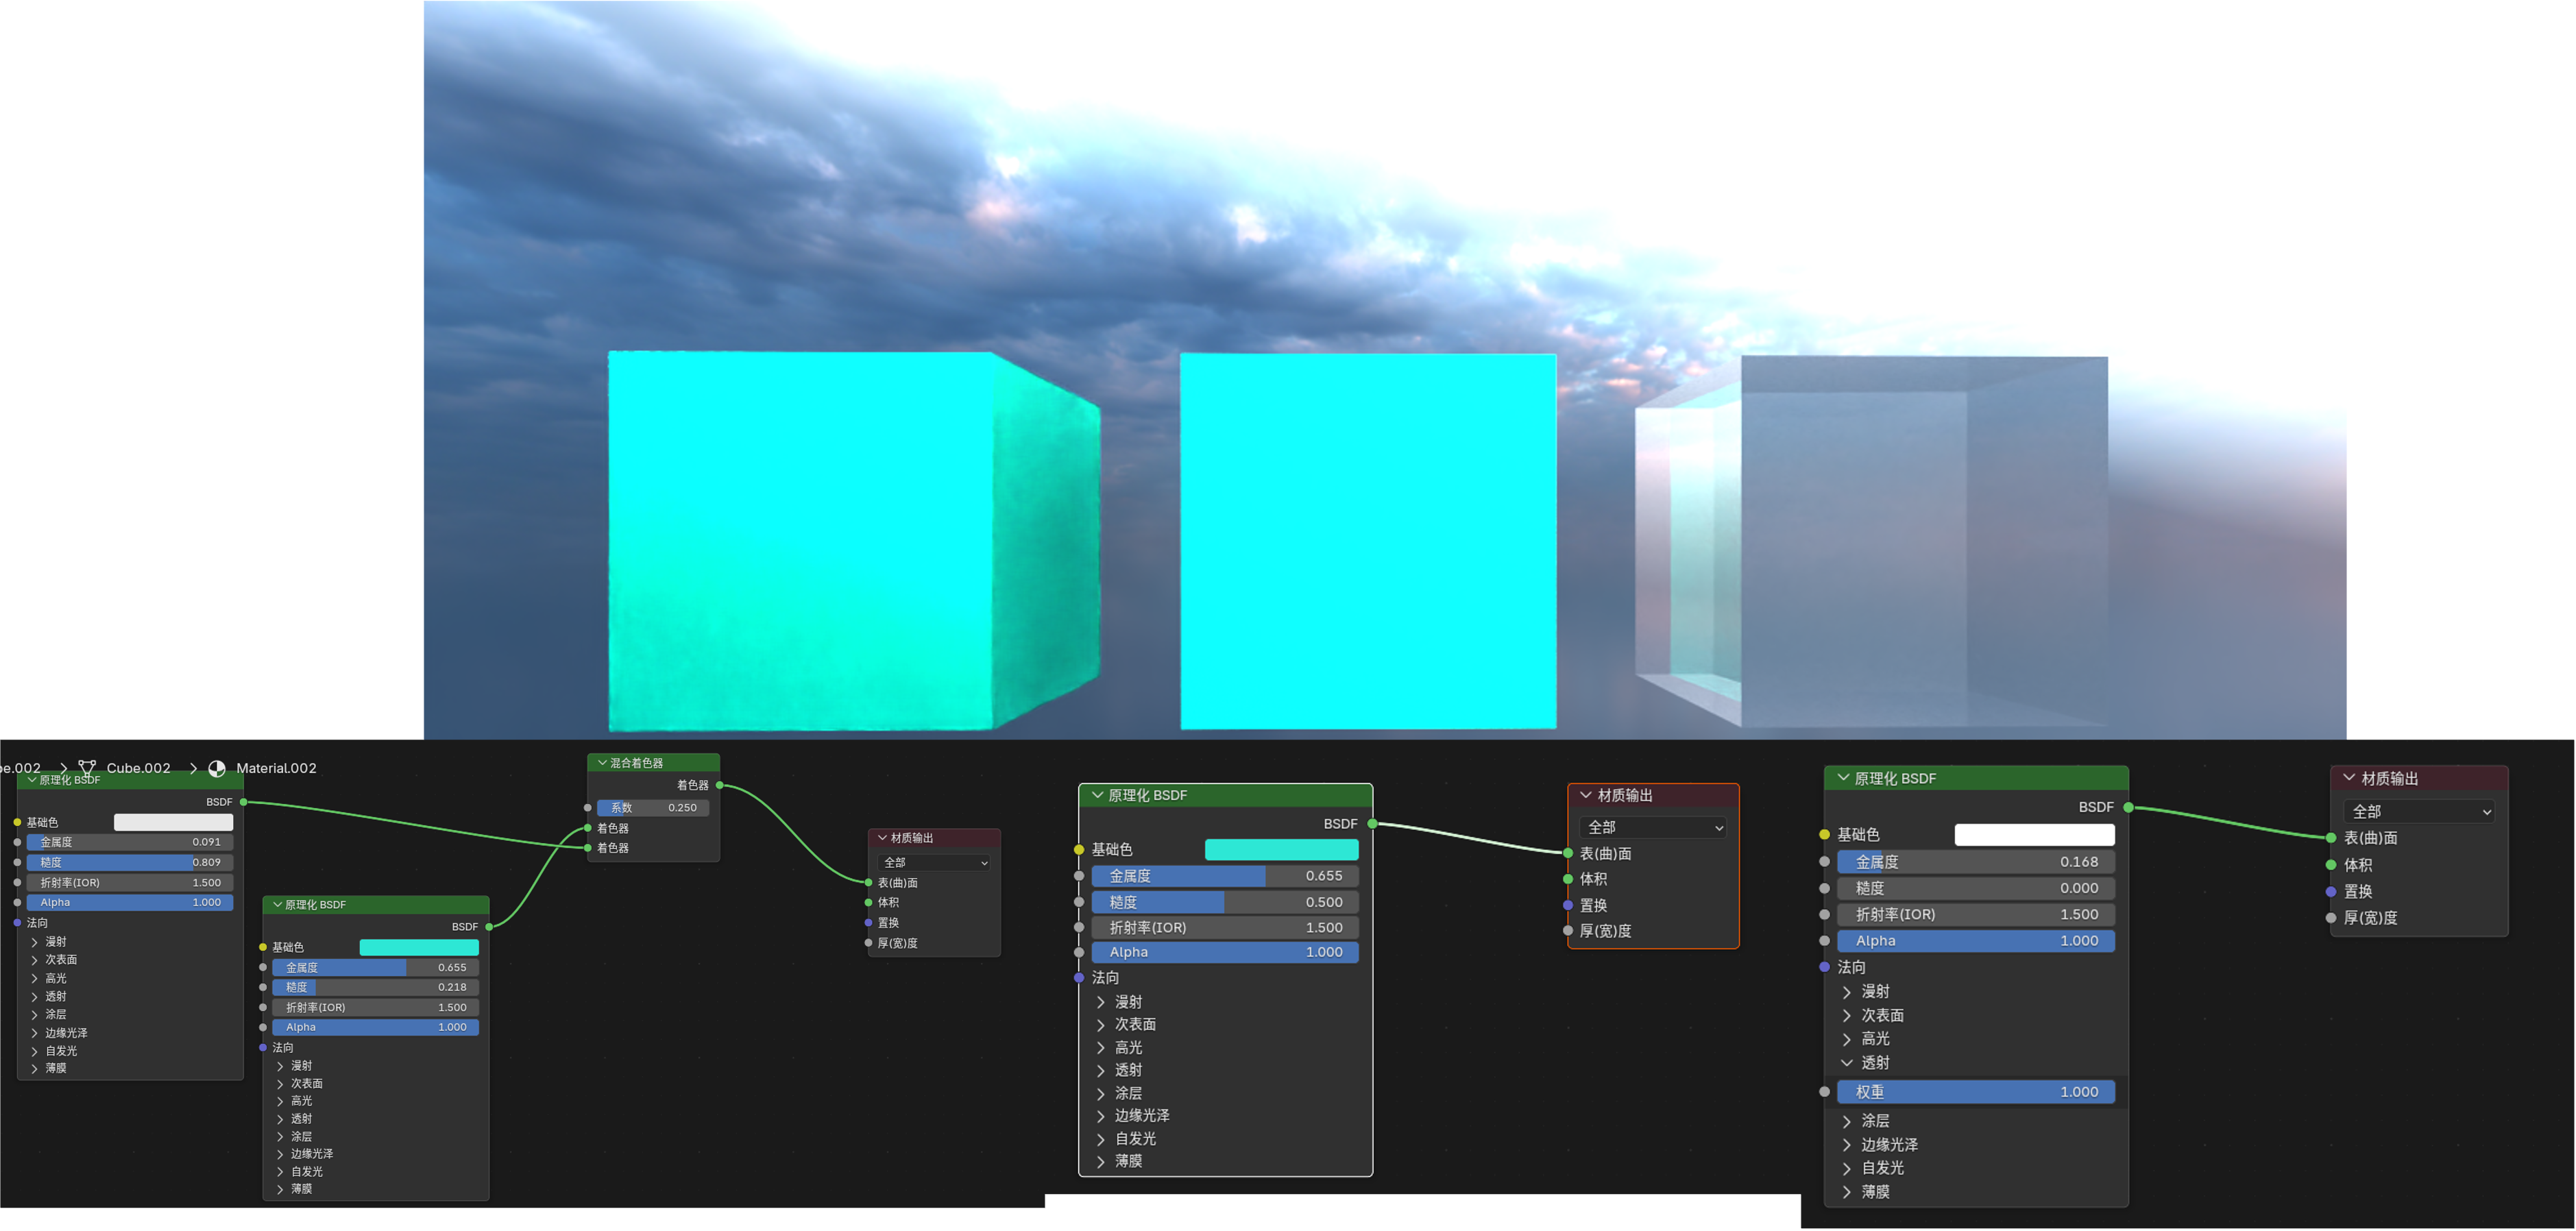
\includegraphics[width=0.9\linewidth]{../slide/fig/cubes2.png}
    \caption{Advanced Materials: Blender's Principled BSDF}
    \label{fig:cubes2}
\end{figure}

\subsection{Large Scene}
We have also tested the renderer with large scenes. Figure~\ref{fig:large_scene} shows the San-Miguel model, which contains 1.7 million triangles and over 200 textures. By using virtual textures, we can handle large scenes with high-resolution textures without overwhelming GPU memory.

\begin{figure}[h]
    \centering
    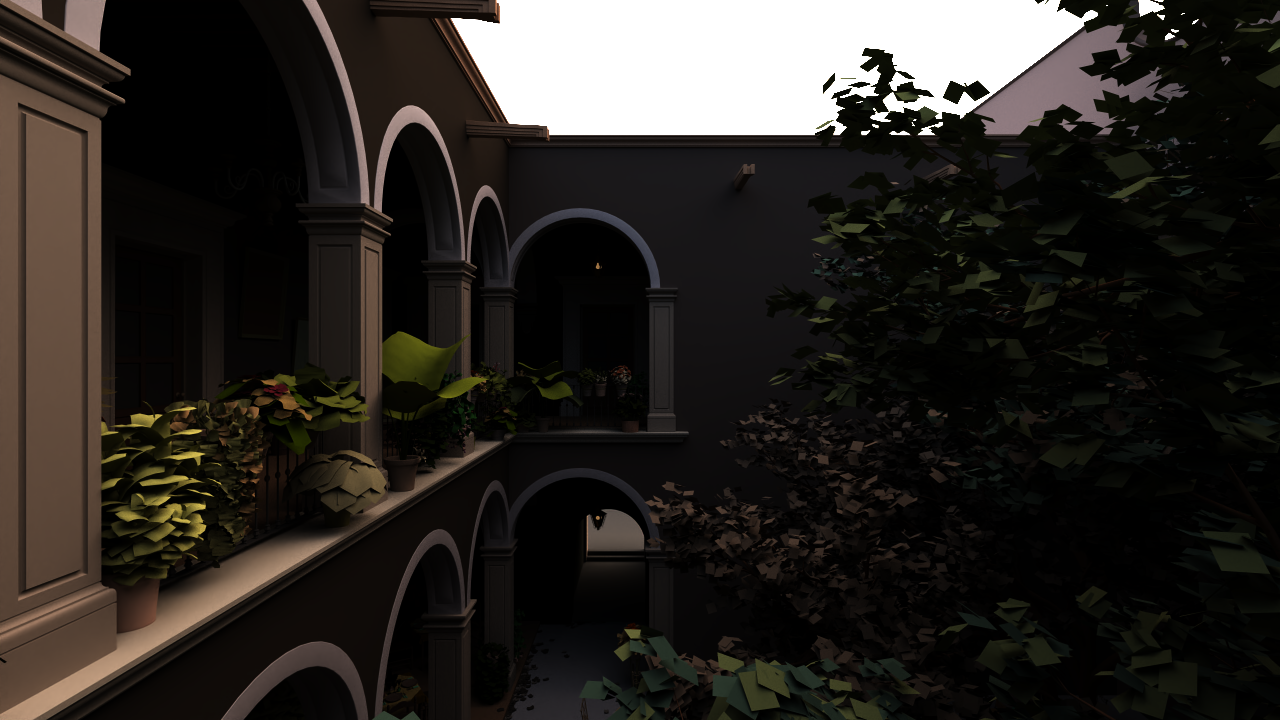
\includegraphics[width=0.8\linewidth]{../slide/fig/large_scene.png}
    \caption{Large Scene Rendering: San-Miguel Model}
    \label{fig:large_scene}
\end{figure}

\subsection{Skybox \& Other Formats}
Figure~\ref{fig:cirno} demonstrates our renderer's capability to utilize skybox images for realistic environmental lighting. The scene features a 3D-scan Cirno fumo model. We have also successfully rendered models from various formats such as glTF and FBX, showcasing the versatility of our system.

\begin{figure}[h]
    \centering
    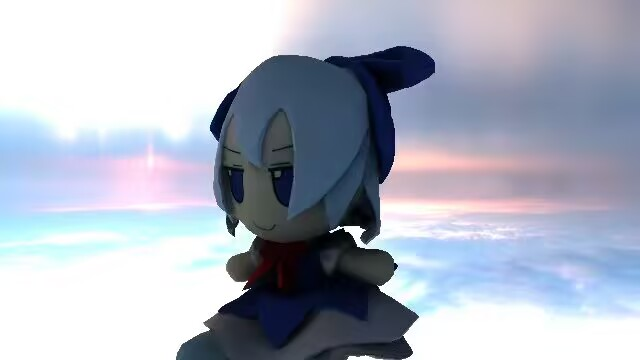
\includegraphics[width=0.8\linewidth]{../slide/fig/cirno.jpg}
    \caption{Skybox Lighting: 3D-scan Cirno fumo scene}
    \label{fig:cirno}
\end{figure}

\subsection{Chromatic Dispersion}
We have implemented the Chromatic Dispersion effect to simulate the phenomenon where light splits into different colors when passing through materials like glass or water. Figure~\ref{fig:chroma} demonstrates this effect.

\begin{figure}[h]
    \centering
    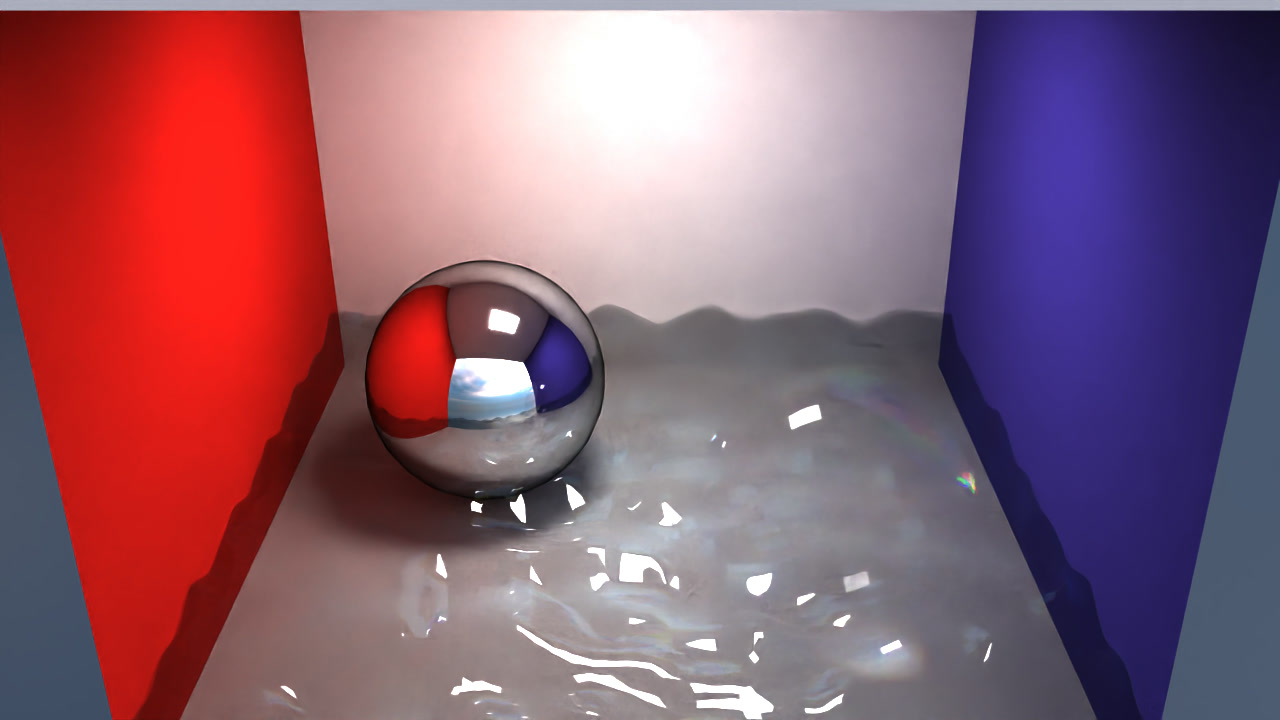
\includegraphics[width=0.6\linewidth]{../slide/fig/chroma.jpg}
    \caption{Chromatic Dispersion Effect}
    \label{fig:chroma}
\end{figure}

\begin{figure}[h]
    \centering
    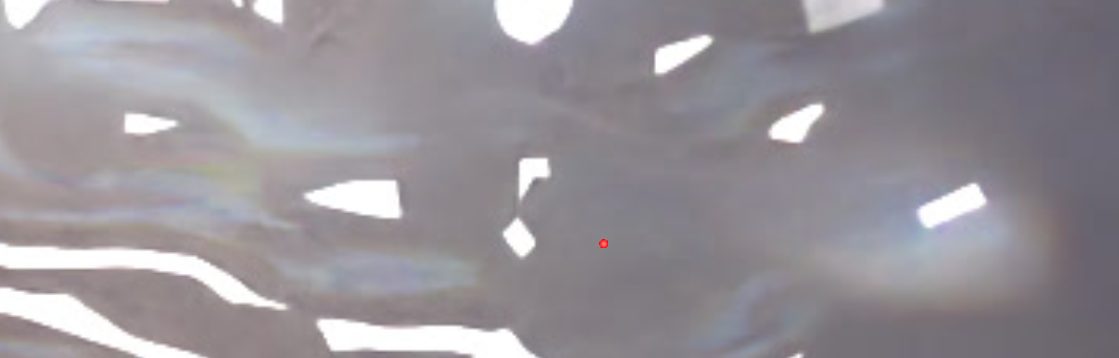
\includegraphics[width=0.75\linewidth]{../slide/fig/chroma-2.png}
    \caption{Chromatic Dispersion: Color fringing on sphere edges}
    \label{fig:chroma2}
\end{figure}

\subsection{Relativistic Rendering}
Our system simulates relativistic visual effects, including aberration, Doppler shift, and the headlight effect. These effects become significant as the camera moves at speeds close to the speed of light.
Figure~\ref{fig:relativity} shows the relativistic effects at different speeds. As the speed increases, the field of view changes (aberration), colors shift (Doppler effect), and brightness varies (headlight effect).

\begin{figure}[h]
    \centering
    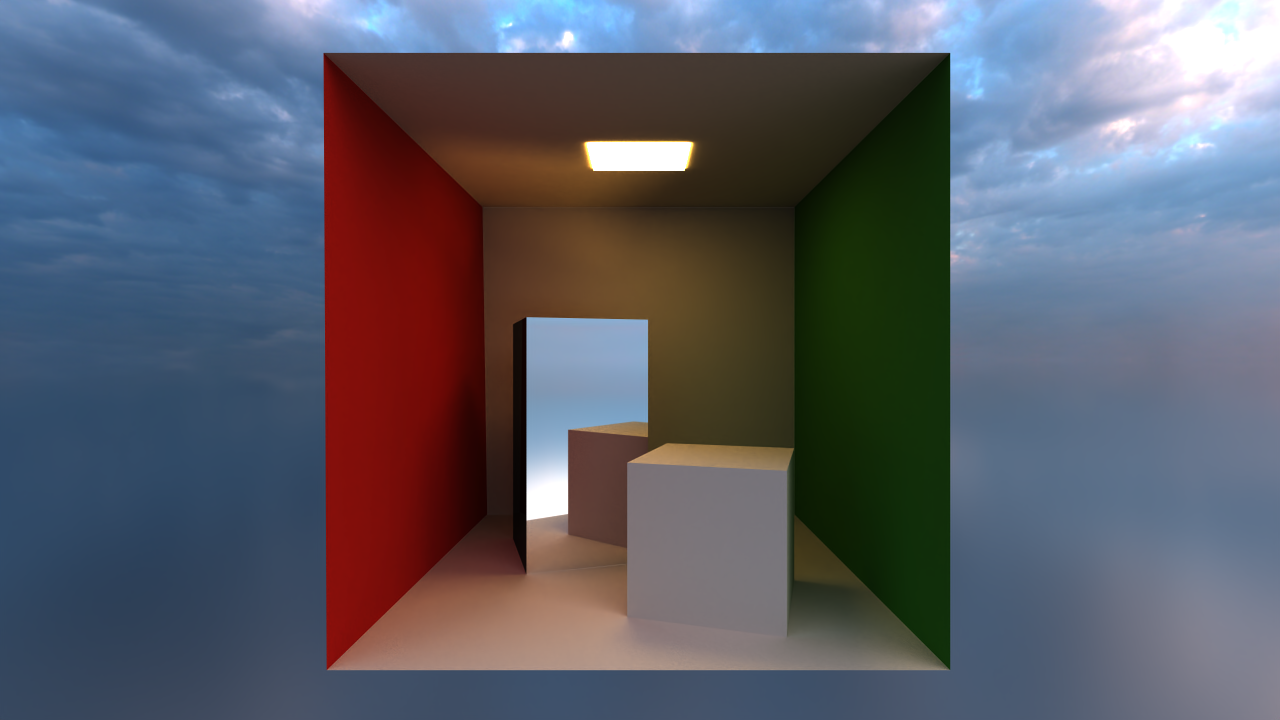
\includegraphics[width=0.45\linewidth]{../slide/fig/0.png}
    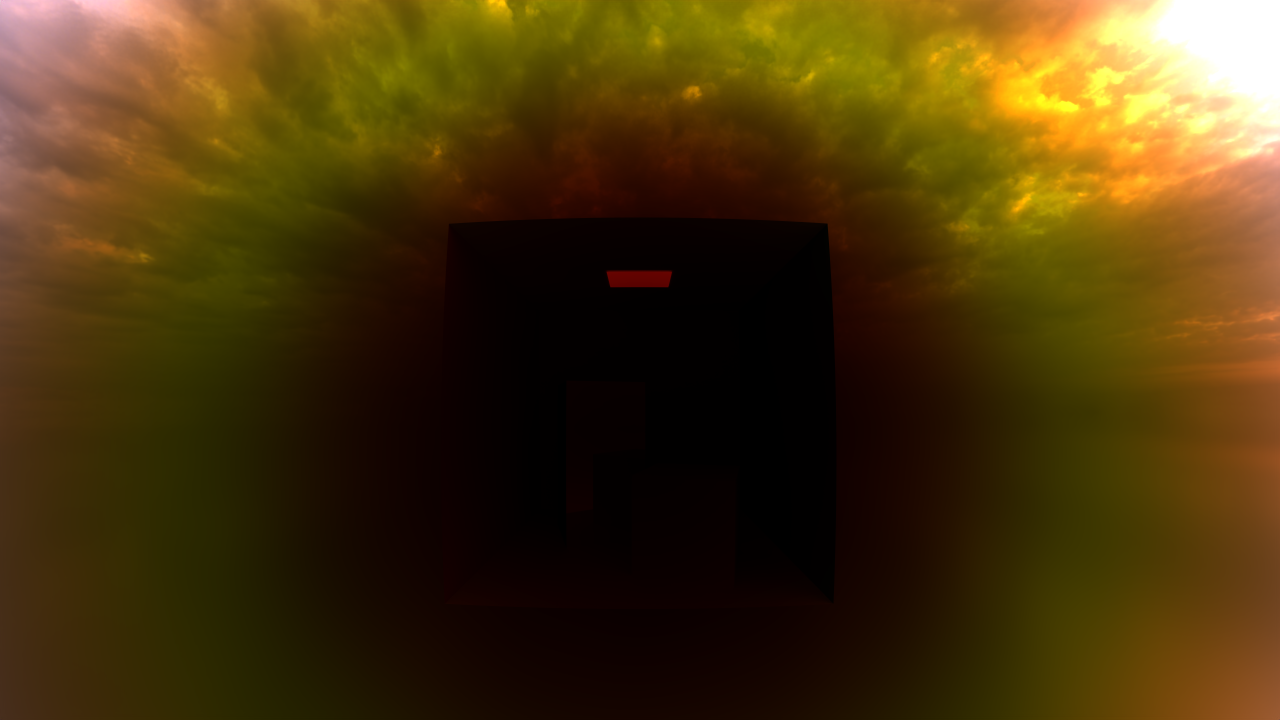
\includegraphics[width=0.45\linewidth]{../slide/fig/4.png}
    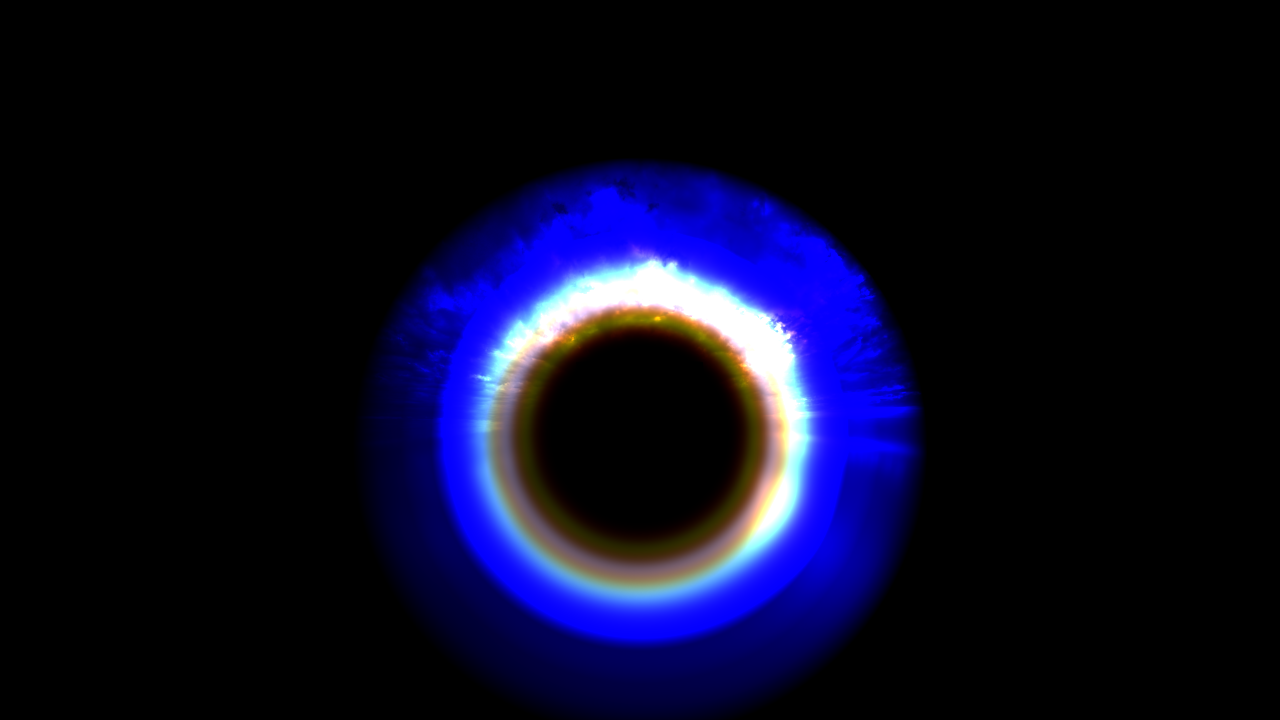
\includegraphics[width=0.45\linewidth]{../slide/fig/9.png}
    \caption{Relativity Effect: Camera moving at 0.0c (Top-Left), 0.4c (Top-Right), and 0.9c (Bottom)}
    \label{fig:relativity}
\end{figure}

\subsection{Depth of Field}
Depth of Field (DoF) is implemented to enhance realism by simulating a camera lens focus. Objects at different distances from the focal point appear blurred. Figure~\ref{fig:dof} shows the DoF effect where the focus is on the center sphere.

\begin{figure}[h]
    \centering
    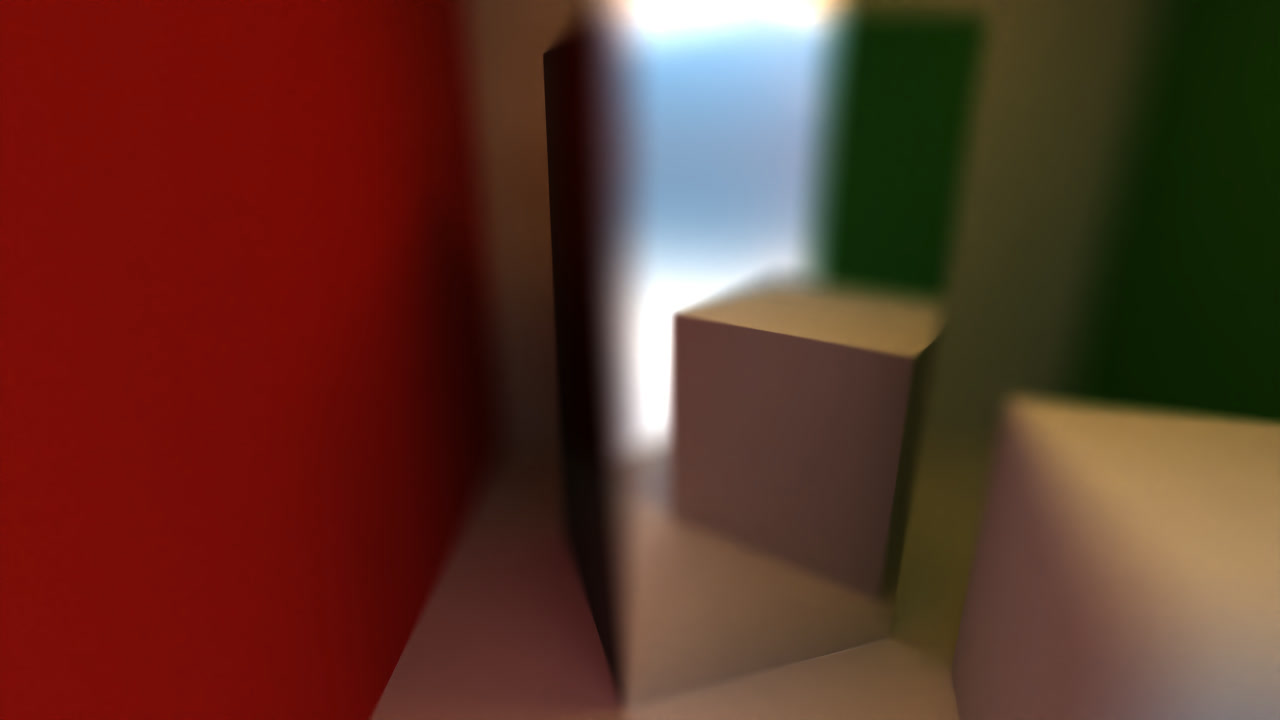
\includegraphics[width=0.5\linewidth]{../slide/fig/depth-of-field.jpg}
    \caption{Depth of Field Effect}
    \label{fig:dof}
\end{figure}

\subsection{Motion Blur}
We have implemented Motion Blur to simulate the blurring of moving objects or the camera itself. This effect adds a sense of speed and dynamism to the rendered scenes. Figure~\ref{fig:motion} displays the motion blur effect.

\begin{figure}[h]
    \centering
    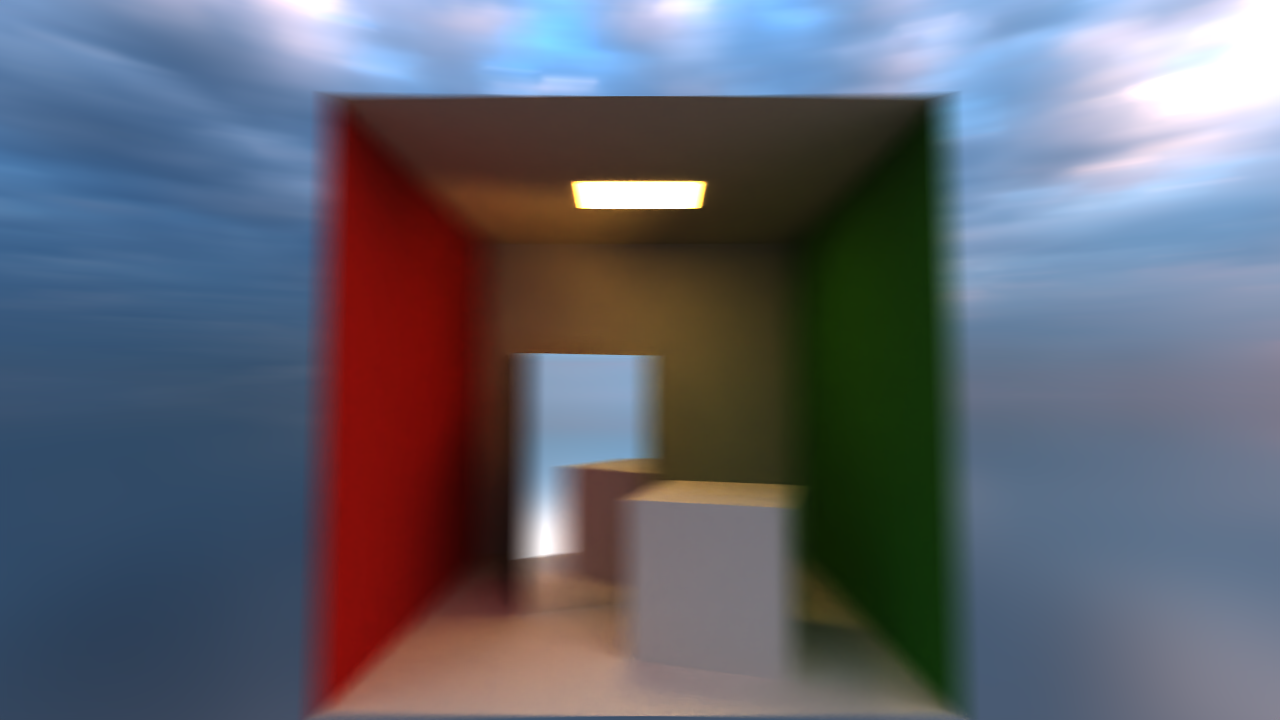
\includegraphics[width=0.8\linewidth]{../slide/fig/motion.png}
    \caption{Motion Blur Effect}
    \label{fig:motion}
\end{figure}

\subsection{Cartoonization}
We implemented a cartoon-style rendering effect characterized by optimized color quantization and smart edge detection. The system increases default quantization levels to 12 for smoother transitions and uses a grayscale gradient method for efficient edge detection. A highlight preservation system is also included to prevent edges from darkening overly bright areas. Figure~\ref{fig:cartoon} shows the cartoonization effect.

\begin{figure}[h]
    \centering
    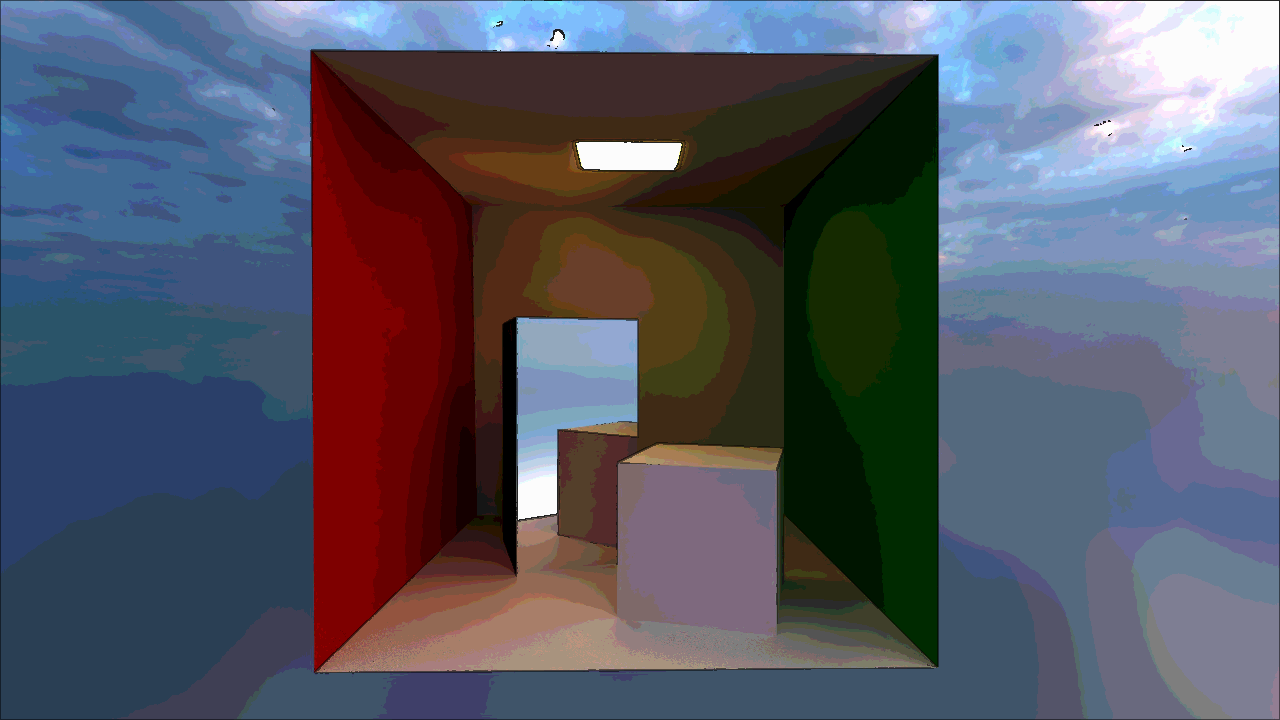
\includegraphics[width=0.8\linewidth]{../slide/fig/cartoon.png}
    \caption{Cartoonization Effect: Cartoon style rendering with optimized color quantization and edge detection}
    \label{fig:cartoon}
\end{figure}

\subsection{Test Scene \& Denoising}
We used the Cornell Box as a test scene to evaluate our denoising implementation. Figure~\ref{fig:denoise} compares the results with and without denoising, both using 100 samples per pixel. The denoising process is highly efficient, taking less than 1 second for a 1920x1080 image, making it suitable for practical use.

\begin{figure}[h]
    \centering
    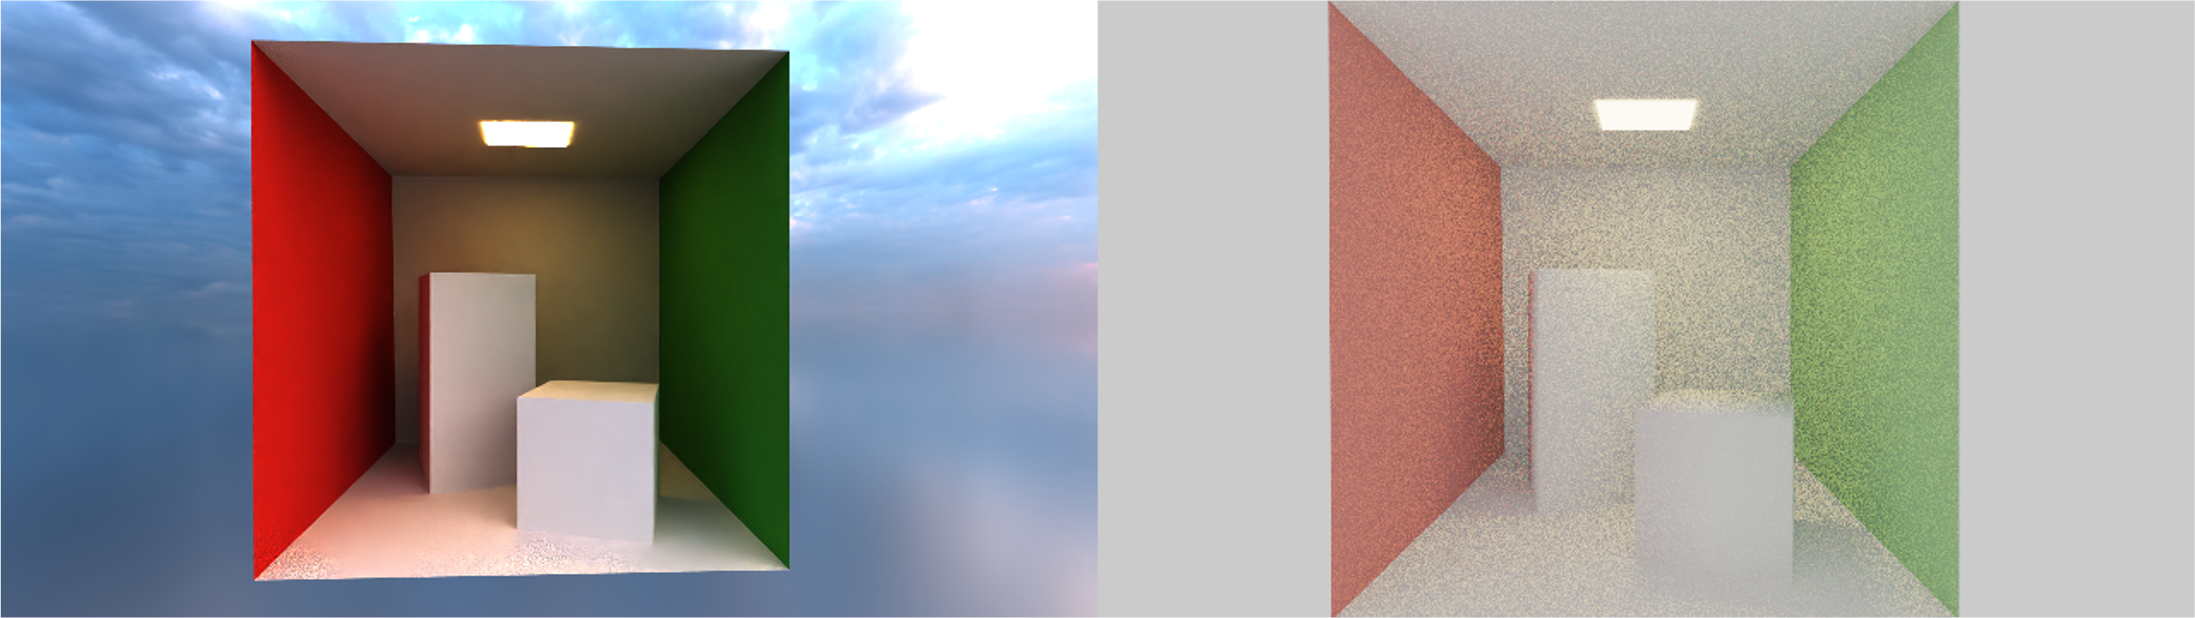
\includegraphics[width=0.9\linewidth]{../slide/fig/denoise.png}
    \caption{Denoising Effect: Left - Denoised, Right - Noisy}
    \label{fig:denoise}
\end{figure}

\subsection{Other Show Cases}
We present additional rendering results to demonstrate the versatility of our system. Figure~\ref{fig:demo2} shows a rendered Breakfast Room scene. Figure~\ref{fig:demo3} displays the Cornell Box with a mirror, highlighting reflection capabilities. Figure~\ref{fig:demo4} presents the Sponza scene, a classic test model for global illumination.

\begin{figure}[h]
    \centering
    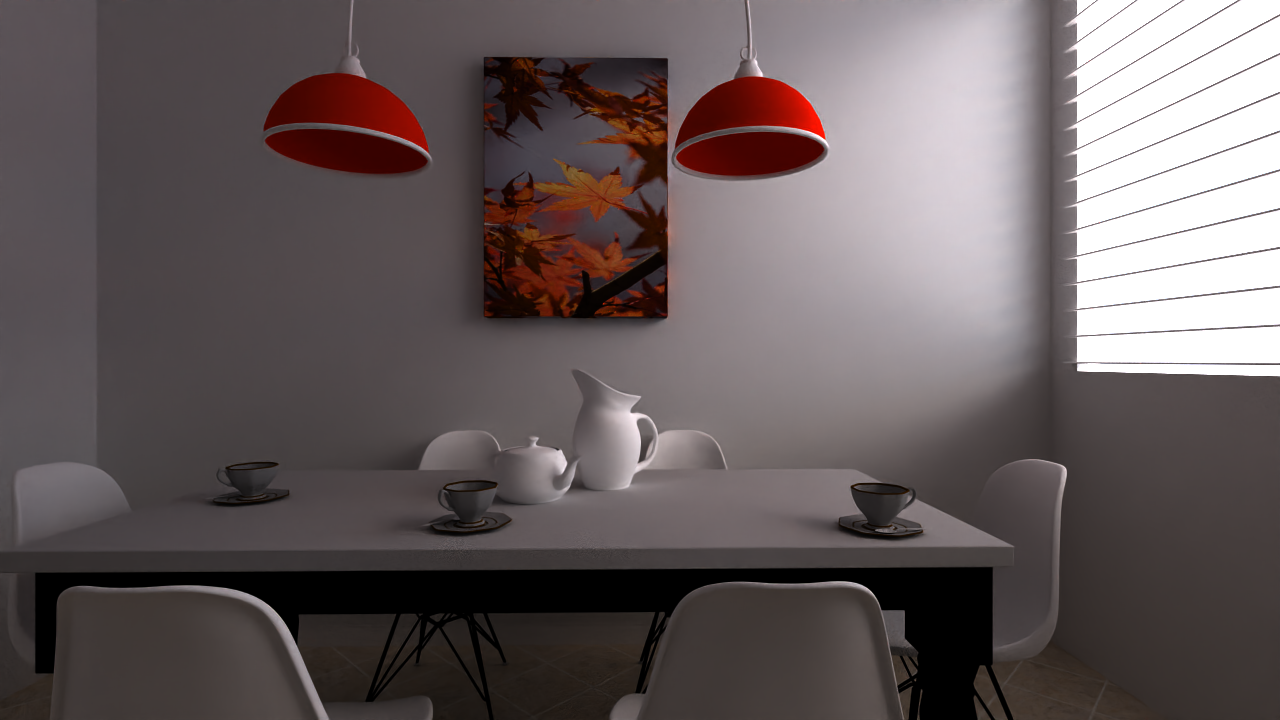
\includegraphics[width=0.9\linewidth]{../slide/fig/demo2.png}
    \caption{Scene: Breakfast Room}
    \label{fig:demo2}
\end{figure}

\begin{figure}[h]
    \centering
    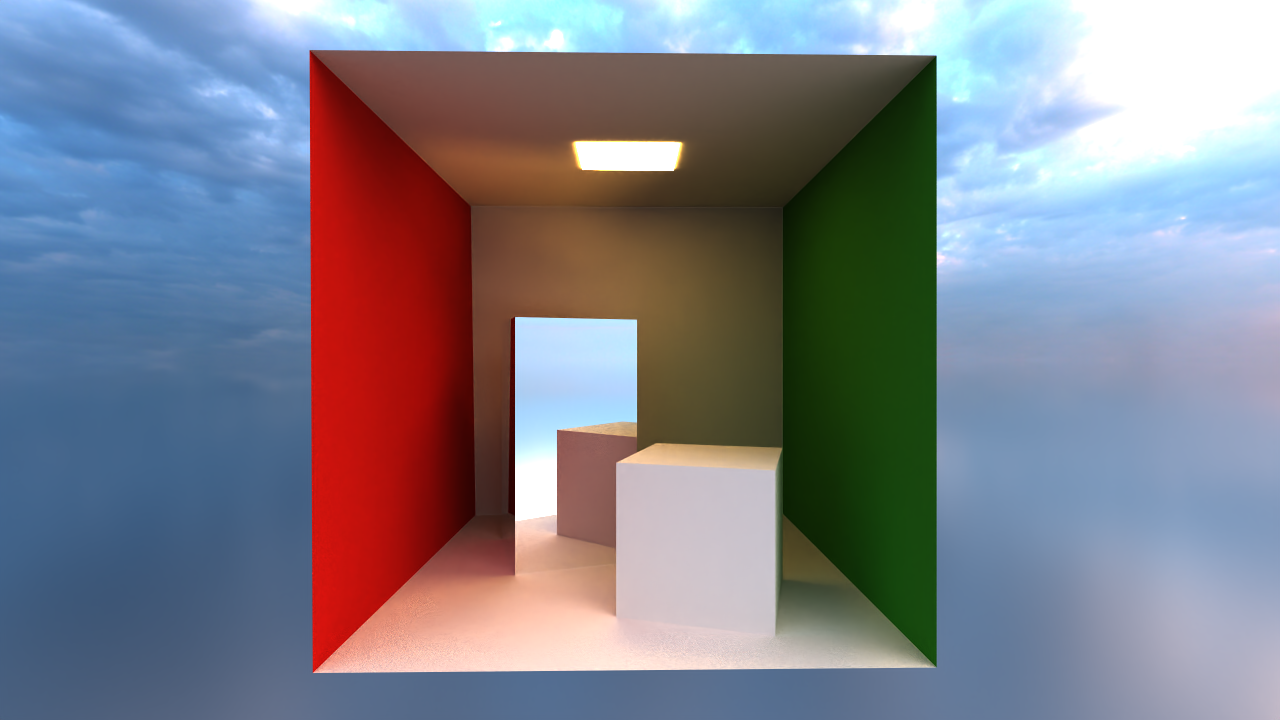
\includegraphics[width=0.9\linewidth]{../slide/fig/demo3.png}
    \caption{Scene: Cornell Box with Mirror}
    \label{fig:demo3}
\end{figure}

\begin{figure}[h]
    \centering
    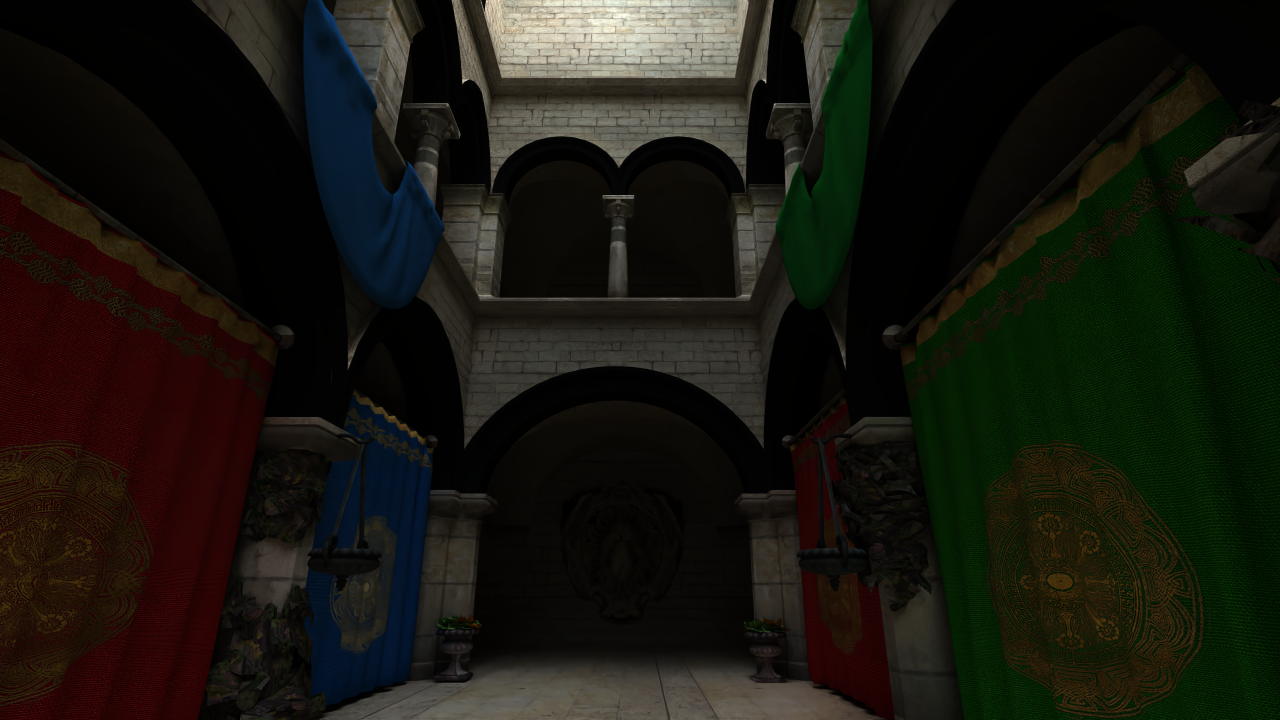
\includegraphics[width=0.9\linewidth]{../slide/fig/demo4.png}
    \caption{Scene: Sponza}
    \label{fig:demo4}
\end{figure}

\section{Discussion}

Our project successfully realized a robust GPU-based rendering system starting from scratch with DirectX 12. We have achieved physically plausible rendering through the implementation of the Disney Principled BSDF, layered materials, and efficient large-scene management using Virtual Textures. The integration of special effects—ranging from cinematic features like Depth of Field and Motion Blur to physical simulations like Relativistic Rendering and Chromatic Dispersion—demonstrates the extensibility of our architecture.

However, several challenges and limitations remain. First, while Virtual Mapping allows rendering large scenes, the page-fault handling mechanism can introduce latency when the camera moves rapidly into new areas. Second, although OIDN effectively removes noise, the raw path tracer still struggles with caustics and small light sources, as our current integrator is uni-directional. Third, relativistic rendering introduces significant variance due to the energy concentration in the headlight effect, often requiring higher sample counts to converge compared to standard scenes.

For future development, we plan to address these limitations through several advanced techniques. Implementing Resampled Importance Sampling (ReSTIR) would significantly improve sampling efficiency for scenes with many dynamic lights. To handle complex light transport and caustics better, we could upgrade the integrator to Bidirectional Path Tracing (BDPT) or Vertex Connection and Merging (VCM). Additionally, extending the renderer to support Participating Media would allow for volumetric effects such as fog and smoke, further enhancing realism. Finally, implementing mesh shaders could provide finer control over geometry processing and culling for massive datasets.

\section{Personal Contribution Statement}
I completed the following course required for extra credit: Tidy and attractive scene creation, including model selection, arrangement, and lighting design, was primarily handled. Principled BSDF, multi-layer material were implemented. Skybox support.

Other work including the path tracing kernel, virtual texture system and relativistic rendering were also developed by me.

\bibliographystyle{ACM-Reference-Format}
\bibliography{references}

\end{document}